% !TEX TS-program = pdflatex
% !TEX encoding = UTF-8 Unicode

% This is a simple template for a LaTeX document using the "article" class.
% See "book", "report", "letter" for other types of document.

\documentclass[11pt]{article} % use larger type; default would be 10pt

\usepackage[utf8]{inputenc} % set input encoding (not needed with XeLaTeX)

%%% Examples of Article customizations
% These packages are optional, depending whether you want the features they provide.
% See the LaTeX Companion or other references for full information.

%%% PAGE DIMENSIONS
\usepackage{geometry} % to change the page dimensions
\geometry{a4paper} % or letterpaper (US) or a5paper or....
% \geometry{margin=2in} % for example, change the margins to 2 inches all round
% \geometry{landscape} % set up the page for landscape
%   read geometry.pdf for detailed page layout information

\usepackage{graphicx} % support the \includegraphics command and options

% \usepackage[parfill]{parskip} % Activate to begin paragraphs with an empty line rather than an indent

%%% PACKAGES
\usepackage{booktabs} % for much better looking tables
\usepackage{array} % for better arrays (eg matrices) in maths
\usepackage{paralist} % very flexible & customisable lists (eg. enumerate/itemize, etc.)
\usepackage{verbatim} % adds environment for commenting out blocks of text & for better verbatim
\usepackage{subfig} % make it possible to include more than one captioned figure/table in a single float
% These packages are all incorporated in the memoir class to one degree or another...

%%% HEADERS & FOOTERS
\usepackage{fancyhdr} % This should be set AFTER setting up the page geometry
\pagestyle{fancy} % options: empty , plain , fancy
\renewcommand{\headrulewidth}{0pt} % customise the layout...
\lhead{}\chead{}\rhead{}
\lfoot{}\cfoot{\thepage}\rfoot{}

%%% SECTION TITLE APPEARANCE
\usepackage{sectsty}
\allsectionsfont{\sffamily\mdseries\upshape} % (See the fntguide.pdf for font help)
% (This matches ConTeXt defaults)

%%% ToC (table of contents) APPEARANCE
\usepackage[nottoc,notlof,notlot]{tocbibind} % Put the bibliography in the ToC
\usepackage[titles,subfigure]{tocloft} % Alter the style of the Table of Contents
\renewcommand{\cftsecfont}{\rmfamily\mdseries\upshape}
\renewcommand{\cftsecpagefont}{\rmfamily\mdseries\upshape} % No bold!

%%% END Article customizations
\setlength{\parindent}{0.0in}
\setlength{\parskip}{0ex}
%\setlength{\headsep}{0.0in}
%\setlength{\topmargin}{0.0in}
%\setlength{\textheight}{8.5in}
%\setlength{\textwidth}{6.0in}
%\setlength{\oddsidemargin}{0.0in}
%\setlength{\evensidemargin}{0.0in}
\geometry{margin=1.0in}

%%% The "real" document content comes below...

\title{Shadow of Evil \\ \Large 4 Player: Pack-a-Punch Round 1}
\author{IMWADI}
%\date{} % Activate to display a given date or no date (if empty),
         % otherwise the current date is printed 

\begin{document}
\maketitle

\section*{Objective}

	The objective of this strategy is to open pack-a-punch and the areas of the map as early and economically as possible, so that less time and effort needs to be spent on each individual task. To do this, it requires cooperation and planning for all four players, each has to strategically use beast modes and all players need to complete rituals together (which is easiest round 1, as the witches are still a 1 knife kill). \\
	\newline
	Please note that as long as players are alive in the ritual room, they will still get points even if they are downed in the process. Make sure to save bullets in your pistols for margwas that will spawn when rituals 2, 4, and opening the PaP are complete. \\
	\newline
	As this is a round 1 strategy, it should go without saying that you should not kill the last zombie (and avoid nukes). I would leave 2 just in case, and it is not really a big deal if a player goes down, accidentally, but trying to continue the strategy on round 2 is significantly more challenging since enemies take more than 1 knife to kill. So prioritize the zombies lives over the players going down, as long as they can still be revived. \\
	\newline
	\emph{No one needs to buy a gun for this, just do not waste bullets from the starting pistol, as you will need it to kill the three magwas that will spawn up.}

\newpage
\section{Easy Street Ritual}

	\emph{Do not immediately use the beast mode.}\\
	
	Before anyone goes beast mode, the first door should be opened. It cost 500 points, and everyone spawns with that much anyway. \\

	Someone will then need to go into beast mode, and complete the following three tasks. Figure \ref{fig:es} shows the tasks that must be completed in beast mode.

	\begin{enumerate}
		\item Destroy the box containing summoning stone.
		\item Charge the crane so the fountain pen is dropped.
		\item Grapple up to the magicians lair, run through it and zap open the stairs to get up there.
	\end{enumerate}

	\begin{figure}[b!]
		\centering
		\subfloat[]{
			\label{fig:es-summon}
			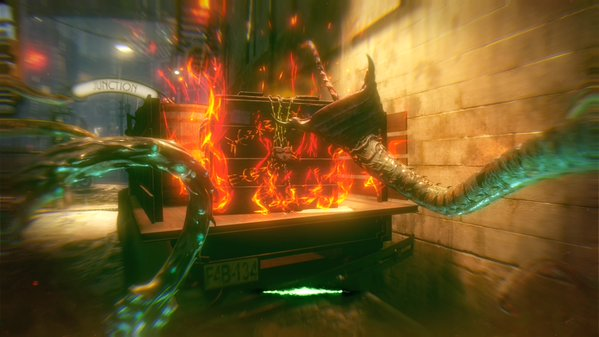
\includegraphics[width=0.475\textwidth]{summoning_key_box.jpg}
		}
		\subfloat[]{
			\label{fig:es-crane}
			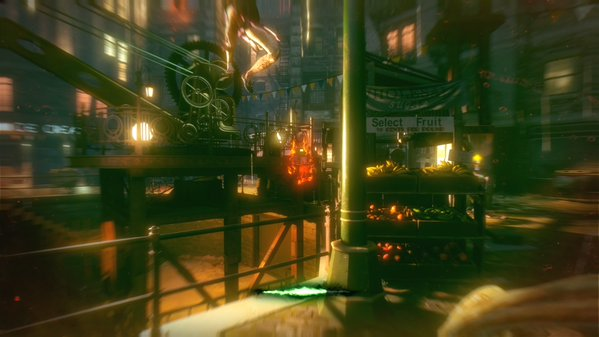
\includegraphics[width=0.475\textwidth]{crane_generator.jpg}
		}
		\hfill
		\subfloat[]{
			\label{fig:es-grapple}
			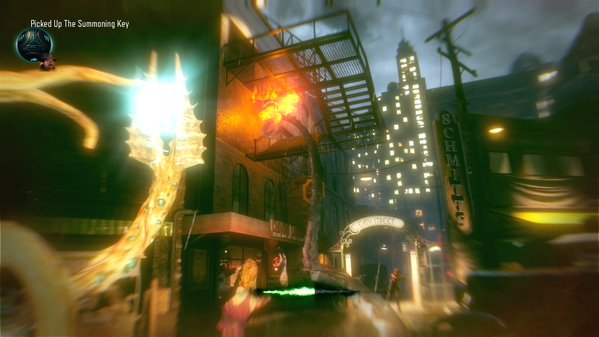
\includegraphics[width=0.475\textwidth]{neros_lair_grapple.jpg}
		}
		\subfloat[]{
			\label{fig:es-stairs}
			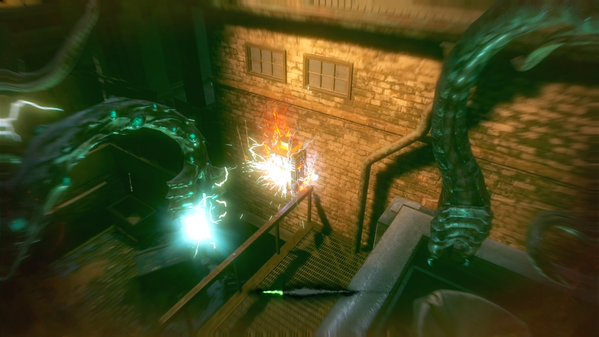
\includegraphics[width=0.475\textwidth]{neros_generator.jpg}
		}
		\caption{
			The tasks that must be completed in beast mode.
			\subref{fig:es-summon} shows the summoning stone box;
			\subref{fig:es-crane} shows the crane that must be powered;
			\subref{fig:es-grapple} shows the grapple point needed to reach Nero's lair;
			and \subref{fig:es-stairs} shows the generator for the stairs.
			}
		\label{fig:es}
	\end{figure}

	Once these actions are complete, one of the players needs to pick up the fountain pen that dropped from the crane. \\

	Next, everyone needs to go into the magicians lair for the ritual. Each player will be rewarded 500 points for completing it, and it will take much less time with everyone in the room anyway. One melee will kill a witch in round 1, so it is quite easy to do. \\

	Finally, someone needs to pick up the gateworm.

\newpage
\section{Waterfront Ritual}

	At this point, three of the players should have over 1000 points (with at least one of them over 1250) and the fourth should have a minimum of 500 (the guy who opened the first door). \\

	The player with the second highest amount of points needs to open the door to the waterfront district. \\

	The player with the most points needs to open the door to the docks, so the boxing gym can be accessed. \\

	The second beast mode then will need to be used to complete these three tasks. Figure \ref{fig:wf} shows the tasks that must be completed in beast mode.

	\begin{enumerate}
		\item Grapple up and melee the box down.
		\item Break open the rift door to the right of where the box fell.
		\item Run down to the gym and break open the door.
	\end{enumerate}

	\begin{figure}[b!]
		\centering
		\subfloat[]{
			\label{fig:wf-box}
			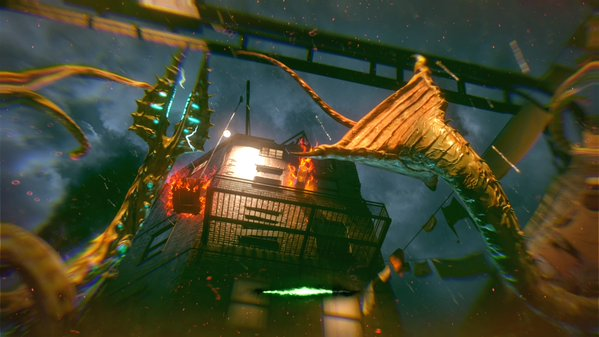
\includegraphics[width=0.475\textwidth]{waterfront_grapple_and_box.jpg}
		}
		\subfloat[]{
			\label{fig:wf-rift}
			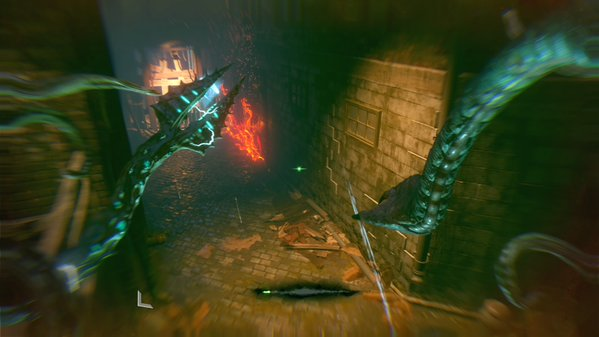
\includegraphics[width=0.475\textwidth]{waterfront_rift_door.jpg}
		}
		\hfill
		\subfloat[]{
			\label{fig:wf-gym}
			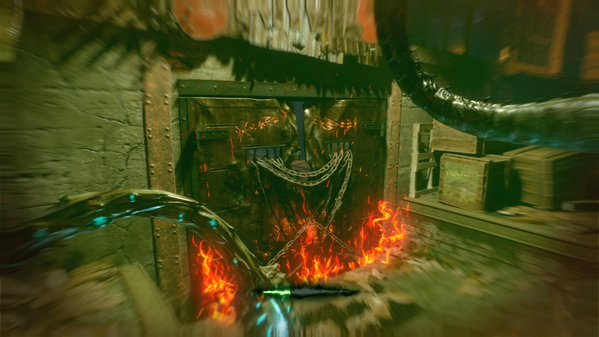
\includegraphics[width=0.475\textwidth]{boxing_gym_door.jpg}
		}
		\caption{
			The tasks that must be completed in beast mode.
			\subref{fig:wf-box} shows the grappling point and box that must be broken;
			\subref{fig:wf-rift} shows the door to the rift that must be broken;
			and \subref{fig:wf-gym} shows the door to the gym that must be broken.
			}
		\label{fig:wf}
	\end{figure}

	Once that is done, someone needs to grab the belt. \\

	Everyone will need to step into the gym and complete the ritual. \\

	Grab the gateworm and kill the margwa.

\newpage
\section{Footlight Ritual}
	
	Now one player should have at least 1500 points, another should have at least 1000, and the last two should have at least 500 (probably more).

	The player with the second highest amount of points needs to open the door to the footlight district. \\

	The player with the most points needs to open the door to the area with all the parked cars, so the burlesque can be accessed. \\

	The third beast mode then will need to be used to complete these two tasks. Figure \ref{fig:fl} shows the tasks that must be completed in beast mode.

	\begin{enumerate}
		\item Grapple up, jump across and melee the box down.
		\item Jump back across and go through to the balcony overlooking the parked car area, and grapple onto the hook on the burlesque building. This will drop you right behind the front sign, where there is a panel that needs to be shocked.
	\end{enumerate}

	\begin{figure}[b!]
		\centering
		\subfloat[]{
			\label{fig:fl-box_grapple}
			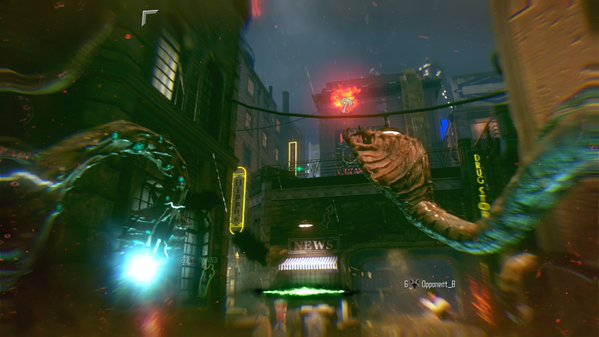
\includegraphics[width=0.475\textwidth]{footlight_box_grapple.jpg}
		}
		\subfloat[]{
			\label{fig:fl-box}
			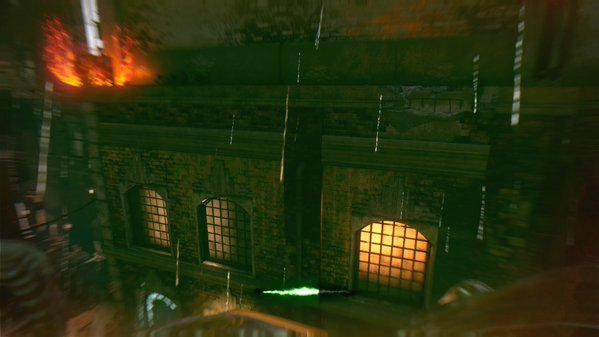
\includegraphics[width=0.475\textwidth]{footlight_box.jpg}
		}
		\hfill
		\subfloat[]{
			\label{fig:fl-door_grapple}
			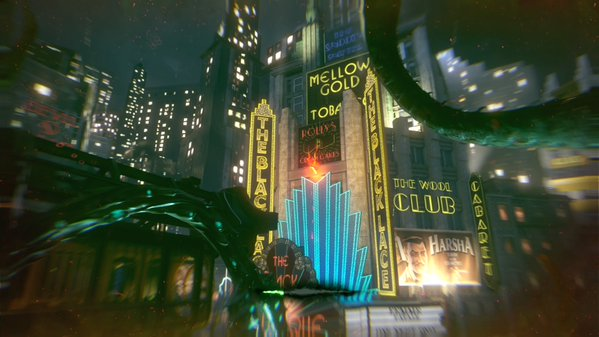
\includegraphics[width=0.475\textwidth]{burlesque_door_grapple.jpg}
		}
		\subfloat[]{
			\label{fig:fl-generator}
			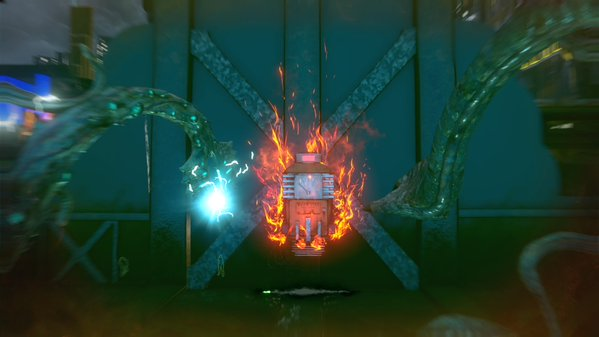
\includegraphics[width=0.475\textwidth]{burlesque_door_generator.jpg}
		}
		\caption{
			The tasks that must be completed in beast mode.
			\subref{fig:fl-box_grapple} shows the grappling point to get up to the box;
			\subref{fig:fl-box} shows the box that must be broken;
			\subref{fig:fl-door_grapple} shows the grapple point needed to reach the door generator;
			and \subref{fig:fl-generator} shows the generator for the burlesque.
			}
		\label{fig:fl}
	\end{figure}


	Once that is done, someone needs to grab the hairpiece. \\

	Everyone will need to step into the burlesque and complete the ritual. \\

	Someone needs to grab the gateworm before leaving.

\newpage
\section{Canal Ritual}
	
	Now two players should have at least 1000 points, with one of them hopefully over 1250. If it is close, 50 points can be earned from repairing a window, or 130 can be earned from melee killing a zombie if you have multiple left. \\

	The player with the second highest amount of points needs to open the door to the canal district. \\

	The player with the most points needs to open the door to the area with the workbench and stairs up to the tram, so the Ruby Rabbit can be accessed. \\

	The final beast mode will need to be grabbed from right next to the build station, and will need to be used to complete these three tasks.

	\begin{enumerate}
		\item Grapple up to the top floor of the ruby rabbit, and go down the two floors to shock the panel and open the stairs.
		\item Jump down into the canal, and head left and shock the panel in the canal wall.
		\item Sprint down the canal, and break the box in the cubby.
	\end{enumerate}

		\begin{figure}[b!]
		\centering
		\subfloat[]{
			\label{fig:cn-grapple}
			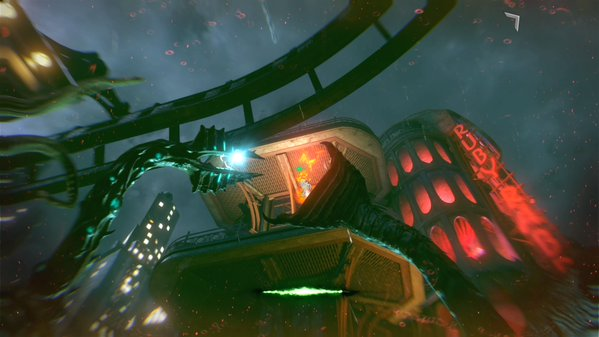
\includegraphics[width=0.475\textwidth]{ruby_grapple.jpg}
		}
		\subfloat[]{
			\label{fig:cn-ruby}
			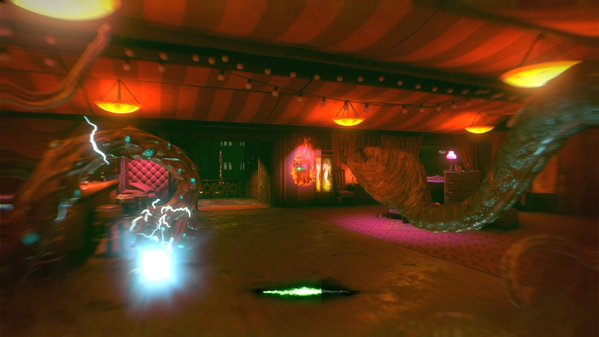
\includegraphics[width=0.475\textwidth]{ruby_generator.jpg}
		}
		\hfill
		\subfloat[]{
			\label{fig:cn-generator}
			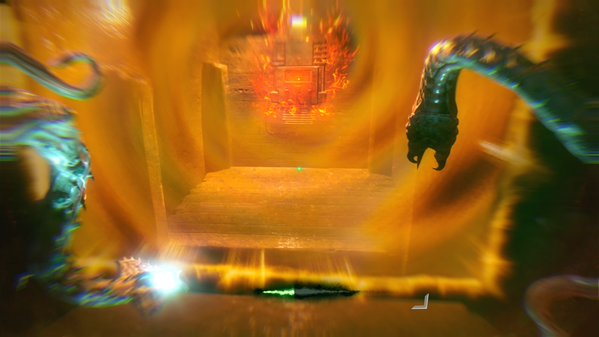
\includegraphics[width=0.475\textwidth]{canal_generator.jpg}
		}
		\subfloat[]{
			\label{fig:cn-box}
			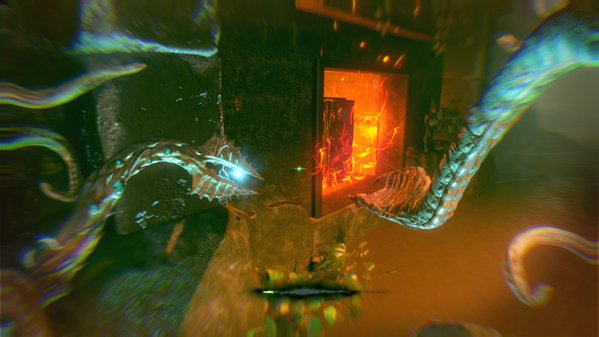
\includegraphics[width=0.475\textwidth]{canal_box.jpg}
		}
		\caption{
			The tasks that must be completed in beast mode.
			\subref{fig:cn-grapple} shows the grapple point to enter the Ruby Rabbit;
			\subref{fig:cn-ruby} shows the generator to open the Ruby Rabbit;
			\subref{fig:cn-generator} shows the generator to open the cage to the badge;
			and \subref{fig:cn-box} shows the box that contains the badge.
			}
		\label{fig:cn}
	\end{figure}


	Once that is done, someone needs to grab the badge. \\

	Everyone will need to step into the second floor of the Ruby Rabbit, and complete the ritual. \\

	At this point, someone needs to grab the gateworm, and then the margwa needs to be killed.

\newpage
\section{The Rift Ritual}

	Now, it is time for all the players to head down to the rift. The door to the portal in the waterfront district should be open. \\

	Once down there, approach the wall with the 5 glowing symbols on them to open up the pack-a-punch chamber. \\

	Each player needs to place the gateworms they picked up in different podiums around the room. \\

	Then approach the table and start the ritual, which will open up pack-a-punch and summon a final margwa. \\

	At this point, each player will have at minimum 1000 points (from the Ruby Rabbit and PaP rituals), so they can ride the tram around to collect the symbols for swords, though all beast modes will be used so eggs will not be able to be grabbed until someone enters the symbols at the beginning of round 2.

		\begin{figure}[h!]
		\centering
		\subfloat[]{
			\label{fig:pap-door}
			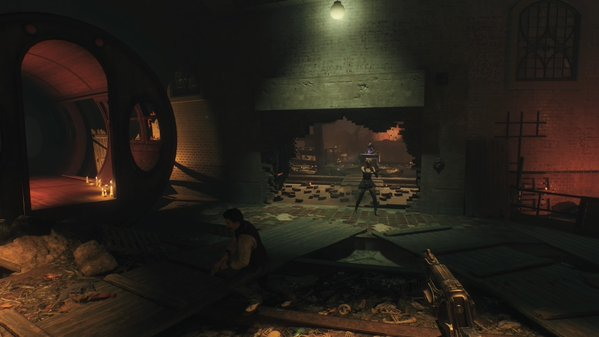
\includegraphics[width=0.475\textwidth]{pap_door.jpg}
		}
		\subfloat[]{
			\label{fig:pap-ritual}
			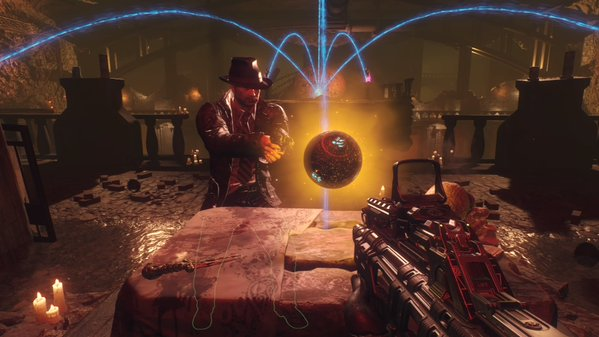
\includegraphics[width=0.475\textwidth]{pap_ritual.jpg}
		}
		\caption{
			The tasks that must be completed in beast mode.
			\subref{fig:pap-door} shows the wall that breaks away and opens up to the Pack-a-Punch;
			and \subref{fig:pap-ritual} shows the gateworms in place and where the ritual is started.
			}
		\label{fig:pap}
	\end{figure}


\end{document}
